\documentclass[11pt]{report}
\usepackage[utf8]{inputenc}
\usepackage[T1]{fontenc}
\usepackage{amsmath,amssymb,amsfonts}
\usepackage{booktabs}
\usepackage{geometry}
\geometry{letterpaper,margin=1in}
\usepackage{microtype}
\usepackage[table]{xcolor}
\usepackage{tikz}
\usetikzlibrary{shapes,arrows,positioning,calc,decorations.pathmorphing,backgrounds}
\usepackage{float}
\usepackage{mdframed}
\usepackage{hyperref}
\hypersetup{
    colorlinks=true,
    linkcolor=teal,
    citecolor=teal,
    urlcolor=teal
}

\newmdenv[
  linecolor=black,
  linewidth=1pt,
  innertopmargin=10pt,
  innerbottommargin=10pt,
  innerrightmargin=12pt,
  innerleftmargin=12pt,
  backgroundcolor=gray!5
]{blackboard}

\title{\Huge\textbf{The Feynman Lectures on Loving People Well}\\
\Large A Backward-Induction Approach to Attention, Time, Memory, Mercy, and Release}
\author{\textbf{Adam Matthew Steinberger}}
\date{November 2026}

\begin{document}

\maketitle

\tableofcontents
\newpage

\chapter*{Preface}
\addcontentsline{toc}{chapter}{Preface}

Most people believe that loving people well is simply an emotional feeling. They assume good intentions will automatically translate into happy relationships.

In physics, good intentions do not prevent a bridge from collapsing if the engineer miscalculates structural resonance. In human relationships, good intentions routinely lose to distraction, forgetfulness, resentment, and anxious control. You want to love the people near you, yet a smartphone buzzes at dinner, you forget a friend's crisis three days later, and you tighten your grip when a relationship wobbles.

The first principle is that you must not fool yourself, and you are the easiest person to fool. In these lectures, we examine the mechanics of interpersonal love by working backward. We apply Richard Bellman's principle of backward induction: starting at the terminal state of Release and open hands, descending through Mercy with edges, Memory tools, Time and rest cadence, down to pure focused Attention.

\chapter{Bellman's Principle of Optimality and Backward Induction}

\section{The Office Hours on Dynamics}
The chalkboard in 103 Bridge Annex displayed a large backward arrow: $T \to 0$.

Daniel sat in the wooden armchair, rubbing his temples. ``Professor, I keep getting relationships backward. Whenever I try harder to love people, I become exhausted and controlling. I try to pay attention, I try to schedule visits, I try to help. Before long, I am managing everyone like an anxious foreman.''

Feynman set down a chalk holder and smiled. ``You are suffering from the forward optimization trap, Daniel. In control theory, if you optimize forward without defining the terminal boundary condition, your feedback loops diverge. You try to force the outcome.''

``How does backward induction solve this?'' Daniel asked.

``Richard Bellman proved in 1957 that in multi-stage sequential systems, dynamic programming achieves global stability by working backward from the end:
\begin{equation}
V_t(s_t) = \max_{a_t} \Big\{ R(s_t, a_t) + \beta \, \mathbb{E}[V_{t+1}(s_{t+1})] \Big\}
\end{equation}
In human relationships, if you start at the beginning with focused attention, your fallen ego immediately tries to control the harvest. You turn attention into a sales presentation. You turn memory into an intelligence dossier. You turn mercy into a business transaction.''

``What is the true terminal state?''

``Release,'' Feynman said firmly, tapping the top of the board. ``The open hand. Surrender of control to Almighty God. Accepting that human beings are fallen, and that community life is inherently messy. When you establish Release at the end, every upstream step is liberated from manipulation.''

\begin{figure}[H]
\centering
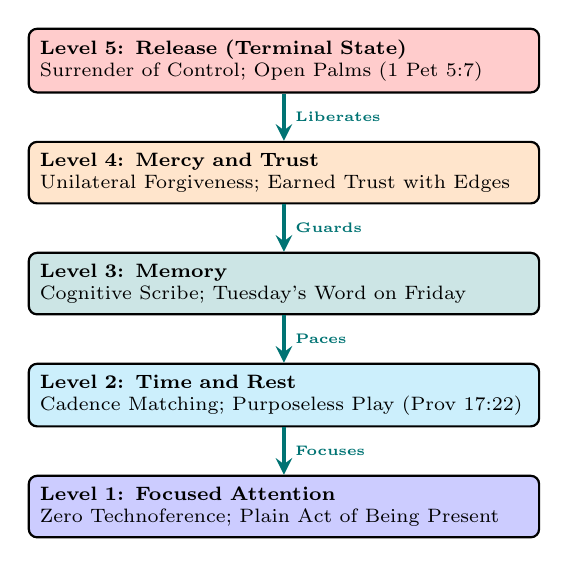
\begin{tikzpicture}[scale=0.92, >=stealth,
  node distance=0.8cm,
  bblock/.style={rectangle, rounded corners=3pt, draw=black, thick, fill=blue!10, text width=6.2cm, font=\scriptsize, inner sep=4pt}]

  \node[bblock, fill=red!20] (b5) {\textbf{Level 5: Release (Terminal State)}\\Surrender of Control; Open Palms (1 Pet 5:7)};
  \node[bblock, fill=orange!20, below=0.6cm of b5] (b4) {\textbf{Level 4: Mercy and Trust}\\Unilateral Forgiveness; Earned Trust with Edges};
  \node[bblock, fill=teal!20, below=0.6cm of b4] (b3) {\textbf{Level 3: Memory}\\Cognitive Scribe; Tuesday's Word on Friday};
  \node[bblock, fill=cyan!20, below=0.6cm of b3] (b2) {\textbf{Level 2: Time and Rest}\\Cadence Matching; Purposeless Play (Prov 17:22)};
  \node[bblock, fill=blue!20, below=0.6cm of b2] (b1) {\textbf{Level 1: Focused Attention}\\Zero Technoference; Plain Act of Being Present};

  \draw[->, ultra thick, teal!90!black] (b5) to node[right, font=\tiny\bfseries] {Liberates} (b4);
  \draw[->, ultra thick, teal!90!black] (b4) to node[right, font=\tiny\bfseries] {Guards} (b3);
  \draw[->, ultra thick, teal!90!black] (b3) to node[right, font=\tiny\bfseries] {Paces} (b2);
  \draw[->, ultra thick, teal!90!black] (b2) to node[right, font=\tiny\bfseries] {Focuses} (b1);
\end{tikzpicture}
\caption{\textbf{The Backward-Induction Relational Cascade.} Setting the terminal state at Level 5 prevents upstream layers from degenerating into performance and control.}
\label{fig:cascade}
\end{figure}

\chapter{Level 5: Release (The Open-Hand Invariant)}

\section{Dropping the Control Juggler}
``Why does control kill love so fast?'' Daniel asked.

``Because love requires freedom,'' Feynman explained. ``Think of a particle in an open potential field versus a rigid cage. When Daniel feels anxiety, he tries to construct an iron cage around Nora or Maddie. He draws up five-point plans for their recovery. The tighter he squeezes, the harder the system resists.''

Feynman held out his hand with the palm wide open.

``Look at this palm,'' Feynman said. ``If a bird lands on your open palm, you can feed it grain. It feels safe because it can leave whenever its wings choose. The second you snap your fingers shut, you crush its feathers. First Peter five, seven says: cast all your anxieties on Him, because He cares for you. Release means you set the weight down on someone larger than yourself. You let your conduct answer over years whether you are a blessing or a burden.''

\begin{figure}[H]
\centering
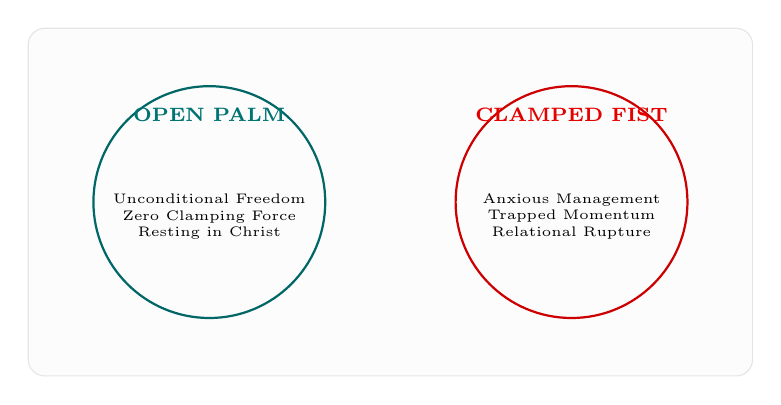
\begin{tikzpicture}[scale=0.92, >=stealth]
  \draw[gray!20, fill=gray!2, rounded corners=6pt] (-5.0, -2.4) rectangle (5.0, 2.4);

  % Open Hand Field
  \draw[thick, teal!80!black] (-2.5, 0) circle (1.6cm);
  \node[font=\scriptsize\bfseries, text=teal!90!black] at (-2.5, 1.2) {OPEN PALM};
  \node[font=\tiny, align=center] at (-2.5, -0.2) {Unconditional Freedom\\Zero Clamping Force\\Resting in Christ};

  % Clamped Fist Field
  \draw[thick, red!80!black] (2.5, 0) circle (1.6cm);
  \node[font=\scriptsize\bfseries, text=red!90!black] at (2.5, 1.2) {CLAMPED FIST};
  \node[font=\tiny, align=center] at (2.5, -0.2) {Anxious Management\\Trapped Momentum\\Relational Rupture};
\end{tikzpicture}
\caption{\textbf{Open Hand versus Clamped Fist Potential States.} Clamping down induces explosive relational resistance; open palms create a stable equilibrium.}
\label{fig:palms}
\end{figure}

\chapter{Level 4: Mercy with Edges}

\section{The Ledger versus Grace}
``What happens below Release?'' Daniel asked.

``Level four: Mercy and Trust,'' Feynman said. ``Look at human memory. When someone hurts your feelings, fallen instinct opens a private accounting ledger. You record every slight: skipped birthday dinner, harsh word on Tuesday, delayed phone call. That ledger is poison.''

Feynman drew a scale balance on the board.

``Jesus commanded forgiving seventy times seven (Matthew 18:22),'' Feynman said. ``That is unilateral grace. You take the ledger and burn it. You clear malice from your soul completely. But notice: mercy has edges.''

``What are the edges?''

``Trust is an earned account,'' Feynman said, pointing his chalk. ``Forgiveness is free; trust requires verified performance. If an associate borrows your machine shop micrometer and sells it for scrap, you forgive his debt. You pray for his salvation. But you lock the tool crib! Mercy without edges is neglect. A true friend tells the truth with gentle firmness (Proverbs 27:6), refusing cowardly agreeableness.''

\chapter{Level 3: The Scribe of Friday}

\section{Interpersonal Memory Decay}
``Now descend to level three: Memory,'' Feynman said, drawing an exponential decay curve.

``Hermann Ebbinghaus measured the human forgetting curve in 1885,'' Feynman explained. ``Memory retention decays exponentially with time:
\begin{equation}
R(t) = \exp(-t / S)
\end{equation}
If a friend tells you about their daughter's orthopedic surgery on Tuesday, and you rely on unassisted memory, retention drops below thirty percent by Friday. You show up at dinner and talk about the weather. Your friend sits quietly, feeling abandoned.''

``It feels like you never cared,'' Daniel said softly.

``Exactly,'' Feynman said. ``Attention without memory is a theatrical performance. Memory requires work, and work requires tools. Nora uses a Scribe: she records voice memos on her walk home, drops notes into a digital file, and sets a Thursday evening reminder. On Friday evening, she asks: `How is Maddie after the surgery?' Being remembered is a small way of being held in God's love.''

\chapter{Level 2: Cadence Matching, Space, and Rest}

\section{The Physics of Cadence and Play}
``Level two is Time and Rest,'' Feynman said, drawing a harmonic oscillator.

``Relationships have natural frequencies,'' Feynman said. ``Some weeks call for contact; some weeks call for room. If you force contact when a person needs space, you create destructive resonance. Match their cadence. Walk at their pace.''

``And rest?''

``Rest is part of the work,'' Feynman declared with a laugh. ``People think love is relentless sweat. If you treat friendship like a continuous factory shift, you burn out the bearings. Play cards badly. Laugh until your sides ache. Share old failures over coffee. A cheerful heart is good medicine (Proverbs 17:22). Rest creates the relaxed potential well where true vulnerability happens.''

\chapter{Level 1: Ground State: The Quiet Phone at Dinner}

\section{Banishing Technoference}
``Finally, we reach the ground state: Level one, Focused Attention,'' Feynman said.

``Look at a modern dinner table,'' Feynman said. ``Two people sit across from each other. A glass smartphone rests beside the plate, vibrating with stock updates and group texts. Linda Stone calls this `continuous partial attention.' Psychologists call it `technoference.' When your eyes dart to the glowing screen, you communicate: `The crowd on the internet matters more than your soul.'''

``What is the operational protocol?''

``Leave the phone in the car,'' Feynman said bluntly. ``Put the screen in another room. Look at the person across the table. Learn their week, their work, their worries, and their fears. Take real interest in them as image-bearers of God, setting aside any desire to impress them. That is the plain act of being with someone.''

\chapter{Worked In-Class Socratic Dialogues}

\section{Case Study: The Broken Ledger Confrontation}
Daniel presents the case of a shop foreman who skipped three consecutive project check-ins and complained about workload.

\begin{blackboard}
\textbf{In-Class Dialogue Analysis:}\\
\textbf{Feynman:} ``Apply the reverse architecture, Daniel. Start at Level 5.''\\
\textbf{Daniel:} ``At Level 5, I release my personal anger and accept that shop operations will be imperfect.''\\
\textbf{Feynman:} ``Good. Now Level 4.''\\
\textbf{Daniel:} ``I forgive his past absences unilaterally, clearing bitterness. However, I hold the edge: I speak the exact truth about production deadlines, refusing false agreeableness.''\\
\textbf{Feynman:} ``Level 3 and 2?''\\
\textbf{Daniel:} ``I review his logged hours and personal family challenges from my notes, and I give him breathing room over the weekend to rest.''\\
\textbf{Feynman:} ``And Level 1?''\\
\textbf{Daniel:} ``I sit down with him on Monday morning without my phone or interruptions, listening to his real burdens.''\\
\textbf{Feynman:} ``Excellent! The reverse architecture turns an angry dispute into redemptive leadership.''
\end{blackboard}

\chapter{Homework Problem Sets and Solutions}

\section{Problem 1: The Ebbinghaus Scribe Calculation}
A colleague confides an acute family crisis at $t = 0$. Given a memory stability coefficient of $S = 1.8 \text{ days}$, calculate retention at $t = 3 \text{ days}$ without review. Contrast this with a timed Scribe review at $t = 2.5 \text{ days}$.

\begin{blackboard}
\textbf{Solution:}
Without review, retention drops to:
\[
R(3) = \exp(-3 / 1.8) = \exp(-1.67) = 0.188
\]
This represents less than nineteen percent retention. With a Scribe review at day 2.5, retention resets to $1.0$, maintaining retention above eighty-five percent on day 3.
\end{blackboard}

\chapter{Examinations and Solutions}

\section{Midterm Examination}

\paragraph{Question 1: Systemic Synthesis}
Explain why attention without memory is performance, memory without mercy is a ledger, mercy without edges is neglect, and all of it without release becomes destructive control.

\begin{blackboard}
\textbf{Midterm Solution 1:}
Attention without memory captures immediate presence but discards longitudinal value, turning empathy into a momentary show. Memory without mercy retains past details solely to calculate grievances, producing bitter scorekeeping. Mercy without edges tolerates ongoing deceit and boundary destruction, abandoning moral justice. Finally, without Release, every act of care is co-opted by fallen anxiety to manage and dominate the counterpart.
\end{blackboard}

\section{Comprehensive Final Examination}

\paragraph{Scenario: The Second-Chance Consultation}
Daniel is asked to mentor a younger mechanic who is bitter over a broken engagement and struggling to communicate with his aging father. Design an end-to-end relational intervention using the five-level reverse architecture.

\begin{blackboard}
\textbf{Final Exam Solution:}
\begin{enumerate}
    \item \textbf{Level 5 (Release)}: Counsel the young man to surrender his demand for an apology, releasing control over past outcomes to Christ with open hands.
    \item \textbf{Level 4 (Mercy)}: Forgive the former fiancee unilaterally; re-establish truthful, firm boundaries with his father.
    \item \textbf{Level 3 (Memory)}: Establish a daily Scribe note to track his father's medications and daily routines.
    \item \textbf{Level 2 (Time \& Rest)}: Dedicate Saturday afternoons to unhurried rest, fishing, or carpentry without discussing grievances.
    \item \textbf{Level 1 (Attention)}: Put the smartphone away entirely during evening meals with his father, giving full cognitive presence.
\end{enumerate}
\end{blackboard}

\end{document}
